\documentclass[a4paper]{scrartcl}
\usepackage{letltxmacro}
\usepackage[T1]{fontenc}
% Use Palatino for serif, Bera Sans for sans serif and Bera Mono for monospace
\usepackage{mathpazo}
\usepackage[scaled=0.86]{beramono}
\usepackage[scaled=0.86]{berasans}
\usepackage{microtype}
% Other convenient packages
\usepackage{xcolor,graphicx,float,caption,nameref,framed,needspace,verbatim,ifdraft}
% tocstyle allows easy styling of the toc, see "Table of Contents" below
\usepackage[tocgraduated]{tocstyle}
% Used to set the section title as part of the page header
\usepackage{scrlayer-scrpage}
% Use normal single quotes in verbatim environment.
% This allows commands to be copies directly into a shell
\usepackage{upquote}
% Make cross-references clickable
\usepackage[hidelinks]{hyperref}

% In draft mode, show frame and mark overfull boxes
\ifdraft {%
  \usepackage{showframe}%
  \overfullrule=5mm%
}{}

% Configure framed package use for code blocks
\colorlet{shadecolor}{lightgray}
\setlength{\OuterFrameSep}{0.2\baselineskip}
\setlength{\FrameSep}{0.2\baselineskip}

% Table of Conents
\usetocstyle{KOMAlike}
\setcounter{tocdepth}{2} % Don't include subsubsection
\settocstylefeature[1]{entryhook}{\normalfont\sffamily\bfseries}
\settocstylefeature[2]{entryhook}{\normalfont\sffamily}
\settocstylefeature[1]{pagenumberhook}{\normalfont\sffamily}
\settocstylefeature[2]{pagenumberhook}{\normalfont\sffamily}

% Page & Fonts
\KOMAoptions{headheight=25pt,footheight=0pt,fontsize=10pt,DIV=11}
\setkomafont{pagination}{\normalfont\sffamily}
\setkomafont{section}{\normalfont\sffamily\bfseries\huge}
\setkomafont{pagehead}{\normalfont\sffamily}
\addtokomafont{labelinglabel}{\bfseries}
\newlength{\headstart}
\setlength{\headstart}{\dimexpr\voffset+1in+\topmargin}
\newlength{\textstart}
\setlength{\textstart}{\dimexpr\headstart+\headheight+\headsep}
\setlength{\textheight}{\dimexpr\paperheight-\textstart-\headstart}
\flushbottom

% Page number
% \rohead is set differently for the title page, and is hence
% setup *after* the title page
\pagestyle{plain.scrheadings}
\lohead[\rightmark]{\usekomafont{section}\rightmark}
\cohead*{}
\cofoot*{}

% Line and page breaking.
\emergencystretch3em
\widowpenalty10000
\clubpenalty10000

% Redefine section command always break the page when
% starting a new section, and to put the section title
% in the page header -- on the first page in the section
% title font, on later pages in the pagehead font
\KOMAoptions{plainheadsepline,headsepline}
\makeatletter
\let\section@orig@phlo\section
\newenvironment{normalsection}%
               {\let\section\section@orig@phlo}%
               {}
\renewcommand\section[1]{%
  % Break page, switch style to use section title font in the header
  \newpage%
  \thispagestyle{scrheadings}%
  % Increment counter
  \refstepcounter{section}%
  % Get section title string, update labels (nameref and numeric)
  \GetTitleString{#1}%
  \let\@currentlabelname\GetTitleStringResult
  \let\@currentlabel\thesection%
  % Add TOC line
  \addxcontentsline{toc}{section}{\texorpdfstring{\sectionformat#1}{\thesection{} #1}}%
  % Update rightmark, this is what will appear in the header
  \markright{\sectionformat#1}%
}
\makeatother

% Prefer page breaks at subsection boundaries -
\makeatletter
\let\subsection@phlo\subsection
\renewcommand\subsection{\needspace{5\baselineskip}\subsection@phlo}
\makeatother

% Environments for shell and R code
\newenvironment{shellcode}%
   {\bgroup\topsep=0.2ex\partopsep=0.2ex\shaded\verbatim}%
   {\endverbatim\endshaded\egroup}
\newenvironment{Rcode}%
   {\bgroup\topsep=0.2ex\partopsep=0.2ex\shaded\verbatim}%
   {\endverbatim\endshaded\egroup}
\newcommand{\shellscript}[1]{\bgroup\topsep=0pt\partopsep=0pt\shaded%
	\verbatiminput{#1}%
	\endshaded\egroup}

% Commands starting with a *d*double-*d*ash (--)
\newcommand{\ddarg}[1]{\texttt{-{}-#1}}

% \version{} and \printversion
\makeatletter
\newcommand{\@version}{}
\newcommand{\version}[1]{\renewcommand{\@version}{#1}}
\newcommand{\printversion}{\@version}
\makeatother

% Print named section references in italic
\makeatletter
\AtBeginDocument{%
  \@ifdefinable{\my@nameref}{%
    \LetLtxMacro\my@nameref\nameref
    \DeclareRobustCommand*{\nameref}[1]{%
      \textit{\my@nameref{#1}}%
    }%
  }%
}
\makeatother

\version{0.9.10}

\begin{document}

% Title. (Last font size in \markright determines distance to headerseprule!)
\thispagestyle{scrheadings}
\markright{\Huge TRUmiCount\hskip0.5em\normalsize\mdseries v \printversion\usekomafont{section}}
\rohead[\today]{\today\usekomafont{section}}

% Table of Contents
\mbox{}\vfill
\begin{normalsection}
\renewcommand*{\contentsname}{User \& Installation Manual}
\tableofcontents
\end{normalsection}
\clearpage

% Put page numbers into top-right corner (where \today went on the first page)
% We switch font at the end to make the baselines of lohead and rohead align
\rohead[\pagemark]{\pagemark\usekomafont{section}}

%\section{Introduction to TRUmiCount}

%XXX Write Me

\section{Installing TRUmiCount}\label{installation}

\subsection{Installation via Conda (Recommended)}

\subsubsection*{Installing Conda}

Conda\footnote{See \url{http://conda.io} for details} allows easy installation of a large range of software packages. See the Conda user guide for installation instructions. Briefly, (on 64-bit Linux) do\footnote{This will install Conda into the directory \texttt{conda} in your home directory. You can replace \texttt{\textasciitilde/conda} with a directory of your choice, but remember to do so everywhere}

\begin{shellcode}
INSTALLER=Miniconda2-latest-Linux-x86_64.sh
curl -O https://repo.continuum.io/miniconda/$INSTALLER
bash $INSTALLER -p ~/conda
\end{shellcode}

\subsubsection*{Creating an environment}

Conda allows creating multiple \emph{environments}, each containing a different collection of packages. We create a separate environment for TRUmiCount

\begin{shellcode}
~/conda/bin/conda create -n trc
\end{shellcode}

This environment is now \emph{activated} to make it the target of further conda commands, and to make the installed software visible. \textbf{This must be done every time you open a new terminal window!}

\begin{shellcode}
source ~/conda/bin/activate trc
\end{shellcode}
%$
\subsubsection*{Installing BioConda}

Conda packages are organized into so-called \emph{channels}. We add the BioConda\footnote{See \url{http://bioconda.github.io/} for details} channel which contains many common bioinformatics tools, amongst which is also TRUmiCount.

\begin{shellcode}
conda config --env --add channels defaults
conda config --env --add channels conda-forge
conda config --env --add channels bioconda
\end{shellcode}

\subsubsection*{Installing TRUmiCount}

With Conda installed and the Bioconda channels added, TRUmiCount is installed with

\begin{shellcode}
conda install trumicount
\end{shellcode}

\subsubsection*{Installing SAMtools and UMI-Tools (Optional)}

TRUmiCount relies on UMI-Tools\footnote{Smith, T.S. \textit{et al.} UMI-tools: Modelling sequencing errors in Unique Molecular Identifiers to improve quantification accuracy. \textit{Genome Research} \textbf{27}, 491-499 (2017). Software available at \url{http://github.com/CGATOxford/UMI-tools}} to extract the UMIs associated with a gene (or other genomic feature) from the mapped reads in a BAM file. We provide a modified version of UMI-Tools that improves the handling of paired-end reads and single-cell data in conjunction with TRUmiCount. You can install our modified version of UMI-Tools with
\begin{shellcode}
conda install -c cibiv umi_tools_tuc
\end{shellcode}
You can also use the unmodified version of UMI-Tools together with TRUmiCount, but will have to manually post-process the output of \texttt{umi\_tools group} before feeding it to TRUmiCount when working with single-cell data. To install the unmodified version, do
\begin{shellcode}
conda install umi_tools
\end{shellcode}

While TRUmiCount does not directly require SAMtools, some of the examples in this manual rely on SAMtools being installed, so we suggest installing them with
\begin{shellcode}
conda install samtools
\end{shellcode}


\subsection{Manual Installation on linux or mac OS}

\subsubsection*{Installing TRUmiCount}

First, make sure you have R\footnote{R Core Team. R: A language and environment for statistical
  computing. R Foundation for Statistical Computing, Vienna, Austria (2017). \url{http://www.R-project.org/}} (at least version 3.1) installed. First, we'll install a few required packages from CRAN. Amogst those is gwpcR\footnote{Pflug, F.P. \& von Haeseler, Arndt. TRUmiCount: Correctly counting absolute numbers of molecules using unique molecular identifiers. \textit{Bioinformatics} (2017). DOI:  \url{http://doi.org/10.1093/bioinformatics/bty283}} which contains the implementation of the model that TRUmiCount relies on. Start R (either on the command line, or open RStudio) and type

\begin{Rcode}
install.packages(c('statmod', 'akima', 'data.table', 'docopt', 'devtools'))
devtools::install_github("Cibiv/gwpcR", ref="latest-release")
\end{Rcode}

Note that unless you have write privileges to your system's R installation, the packages will be installed only for your user.

With all prerequisites now available, TRUmiCount can now be installed. The commands below install TRUmiCount into your home directory. To install TRUmiCount system-wide (assuming you have the necessary privileges), don't specify \ddarg{prefix \textasciitilde/.local}.

\begin{shellcode}
git clone https://github.com/Cibiv/trumicount.git trumicount
cd trumicount/
mkdir -p ~/.local/bin
./install.R --prefix ~/.local
\end{shellcode}

To be able to run TRUmiCount, you must add \texttt{\textasciitilde/.local/bin} to your \texttt{PATH}. \textbf{This must be done every time you open a new terminal window!}

\begin{shellcode}
export PATH=~/.local/bin:$PATH
\end{shellcode}
%$

\subsubsection*{Installing UMI-Tools}

TRUmiCount uses UMI-Tools\footnote{Smith, T.S. \textit{et al.} UMI-tools: Modelling sequencing errors in Unique Molecular Identifiers to improve quantification accuracy. \textit{Genome Research} \textbf{27}, 491-499 (2017). Software available at \url{http://github.com/CGATOxford/UMI-tools}} to extract UMIs from mapped reads and to correct for sequencing errors within the UMIs. We provide a modified version of UMI-Tools that improves the handling of paired-end reads and single-cell data in conjunction with TRUmiCount. You can install our modified version of UMI-Tools with

\begin{shellcode}
URL=https://github.com/Cibiv/UMI-tools.git
git clone -b tuc_patches $URL umi_tools
cd umi_tools
python setup.py install --user
\end{shellcode}
%$

To install the original version, instead do
\begin{shellcode}
URL=https://github.com/CGATOxford/UMI-tools
git clone $URL umi_tools
cd umi_tools
python setup.py install --user
\end{shellcode}

Note that you will then have to manually post-process the output of \texttt{umi\_tools group} before feeding it to TRUmiCount when working with single-cell data.

\clearpage
\subsection{Running TRUmiCount}

After installing TRUmiCount, you can display a list of options with

\begin{shellcode}
trumicount --help
\end{shellcode}

For a detailed explanation of TRUmiCount's various modes of operation and supported file format, see \nameref{using-trumicount} and \nameref{parameter-reference}.

You can download an example input file\footnote{containing a reduced version, restricted to the first 1000 genes and sub-sampled to 50\%, of RNA-Seq data published in Kivioja, T. \textit{et al.} Counting absolute numbers of molecules using unique molecular identifiers. \textit{Nature Methods} \textbf{9}, 72-74 (2011)} in BAM format and index it (necessary for reading it with TRUmiCount) with

\begin{shellcode}
curl -O https://cibiv.github.io/trumicount/kv_1000g.bam
samtools index kv_1000g.bam
\end{shellcode}

From the indexed BAM file, you can let TRUmiCount compute a table containing the bias-corrected number of transcript molecules for each gene and write it to \texttt{kv\_1000g.tab} with

\shellscript{../examples/kv_1000g.min.cmd}

For more examples of how to use TRUmiCount and a discussion of the various options used here, see \nameref{examples}.

\section{Using TRUmiCount}\label{using-trumicount}

\subsection{Input formats \& options}\label{input-options}

To be able to separate true UMIs from phantoms and to estimate and correct for the percentage of true UMIs that are lost during library preparation or data processing, TRUmiCount analyses the distribution of read counts per UMI for each gene (or any other type of genomic feature). TRUmiCount by default assumes that

\begin{itemize}
  \item Each UMI initially had two copies. This is e.g. the case if molecules before amplification were double-stranded and the copies produced from both strands are identical. This number can be changed with ``\ddarg{molecules}''
  \item UMIs must be supported by at least two reads to be assumed to be a true UMI and not a phantom. This threshold can be changed with ``\ddarg{threshold}''.
\end{itemize}

\subsubsection*{Reading UMIs from a BAM File}\label{input-bam}

If a mapped BAM File is provided as input with ``\ddarg{input-bam}'', TRUmiCount uses UMI-Tools' ``\texttt{group}'' tool to extract a list of UMIs and their read counts from the specified BAM file. Sequencing errors within the UMIs are corrected by UMI-Tools by \emph{merging} similar UMIs into one. When reading BAM file, on top of the defaults mentioned above, UMI-Tools assumes that
\begin{itemize}
  \item The BAM file must have a corresponding index. A suitable index can be created with ``\texttt{samtools index} \textit{bamfile}''.
  \item Sequences names are gene names. With the ``\ddarg{gene-tag}'' option, gene names can be read from a \emph{tag} instead, whose name is specified with ``\ddarg{umitools-option} \allowbreak\ddarg{gene-tag=}\allowbreak\textit{tagname}''.
  \item The UMI was appended to the read name, separated by `\_'. A different separator can be specified with ``\ddarg{umi-sep}''
  \item The BAM file contains single-end reads (read2 is ignored). To take the mapping position of both mates into account when grouping reads by UMI, specify ``\ddarg{paired}''.
  \item Reads with a mapping quality below 20 should be ignored. This threshold can be changed with ``\ddarg{mapping-quality}''.
\end{itemize}

\subsubsection*{Reading unfiltered UMIs from a tab-separated file}

Instead of using UMI-Tools to extract UMI and their read counts from a BAM file, TRUmiCount is also able to read a previously computed table of UMIs with ``\ddarg{input-umis}'' (see \nameref{output-options} for how to generate such a table). The table must be tab-separated with one row per UMI and contain at least the columns ``sample'', ``gene'', ``reads''. Similar UMIs are assumed to already have been merged, but filters are assumed \emph{not} to have been applied yet. When dealing with strand UMIs (see section \nameref{strand-umis}), TRUmiCount also requires the columns ``pos'' and ``end'', which contain the mapping position of read1 respectively read2.

The UMI-Tools and BAM-related options ``\ddarg{umi-sep}'', ``\ddarg{umitools}'', ``\ddarg{umitools-option}'', ``\ddarg{paired}'' and ``\ddarg{mapping-quality}'' are ignored if ``\ddarg{input-umis}'' is used.

\subsection{Output formats \& options}\label{output-options}

\subsubsection*{Writing corrected per-gene molecule counts to a tab-separated file}

The main output of TRUmiCount is a table, written to a tab-separated file specified with ``\ddarg{--output-counts}'' containing for each gene the columns
\needspace{5\baselineskip}
\begin{labeling}[:]{efficiency\ }
\item[sample] The sample identifier (e.g cell barcode)
\item[gene] The gene identifier (see discussion in \nameref{input-bam})
\item[n.umis] The number of true UMIs (i.e. after applying filters) detected
\item[n.tot] The estimated total number of molecules, i.e. ``n.umis'' / (1 - ``loss'').
\item[efficiency] The estimated gene-specific amplification efficiency
\item[depth] The gene-specific sequencing depth in reads/molecule.
\item[loss] The estimated gene-specific loss, i.e. the probability of not detecting or filtering a true UMI.
\item[n.obs] The number of observations used to estimate ``efficiency'', ``depth'' and ``loss''. If ``\ddarg{combine-strand-umis}'' is used, this number can be larger than ``n.umis'', because in this case ``n.umis'' counts UMI \emph{pairs} while ``n.obs'' counts \emph{strand} UMIs.
\end{labeling}

\subsubsection*{Writing unfiltered UMIs to a tab-separated file }

The option ``\ddarg{output-umis}'' (together with ``\ddarg{input-bam}'') writes the UMIs reported by UMI-Tools (after merging similar UMIs) and their read counts to a tab-separated file, suitable for being later read with ``\ddarg{input-umis}''. This can be used to avoid the overhead of running UMI-Tools multiple times if the same input BAM file is processed multiple times with TRUmiCount, e.g. to test different read count thresholds or initial molecule counts.

\subsubsection*{Writing final, filtered \& strand-combined UMIs to a tab-separated file }

The final list of UMIs used when fitting the model and computing corrected molecule counts can be output with ``\ddarg{output-final-umis}''. The format of the generated file depends on whether one of ``\ddarg{filter-strand-umis}'' or ``\ddarg{combine-strand-umis}'' is used. In the former case, the table contains one line per \emph{strand UMI}, listing the UMI's read count in the column ``reads'' and it's partner UMI's read count in ``reads.other''. In the latter case, the table contains one line per \emph{UMI pair}, listing the read count of the plus-strand partner UMI (arbitrarily chosed to be the one where read1's mapping position is smaller than read2's) in ``reads.plus'' and the read count of the minus-strand partner UMI in ``reads.minus''.

\subsubsection*{Diagnostic Plots}

When the ``\ddarg{output-plots}'' option is used, TRUmiCount generates diagnostic plots as part of the analysis and writes them to the specified PDF file. The plots produced are

\begin{description}
\item[Distribution of reads per UMI.] This plot shows the observed library-wide distribution of per-UMI read counts and the distribution predicted by TRUmiCount's model of amplification and sequencing.

\item[Variance of the gene-specific loss estimate.] Shows the observed variance of the gene-specific loss estimates as a function of the number of UMIs per gene ($n_{\textrm{\tiny obs}}$) and compares it to the interpolation curve ($s + u / n_{\textrm{\tiny obs}}$).
\end{description}

\subsection{Strand UMIs}\label{strand-umis}

Some UMI-based library preparation protocols produce \emph{strand UMIs} where the two strands of an initial double-stranded template molecule produce distinct (but related) UMIs. Filtering out UMIs for which the partner UMI corresponding to the second strand is not detected offers a second possibility (besides the read count threshold) for filtering our phantom UMIs.

TRUmiCount supports stranded UMIs as produced by the protocol of Shiroguchi \textit{et al.}\footnote{Shiroguchi, K., Jia, T. Z., Sims, P. A. \& Xie, X. S. Digital RNA sequencing minimizes sequence-dependent bias and amplification noise with optimized single-molecule barcodes. \textit{Proceedings of the National Academy of Sciences of the United States of America} \textbf{109}, 1347-1352 (2012).}. With this protocol, both read1 and read2 carry a separate molecular barcode. UMI pairs belonging to the same double-stranded template molecule are found by looking for pairs of UMIs whose read1 and read2 barcodes and mapping positions are swapped (mapping position here refers to the genomic coordinate of the first mapped base in \emph{read direction}, i.e. for reverse-mapped reads this differes from the mapping position stated in the BAM file).

When working with strand UMIs, the initial molecule count should usually be set to 1 (the default is 2!), i.e. ``\ddarg{molecules 1}'' should be used.

\subsubsection*{Filtering out incomplete strand UMI pairs}

With the option ``\ddarg{filter-strand-umis}'', UMIs are filtered out if their partner UMI cannot be detected (these UMIs are also not counted as ``phantom UMIs'' in the diagnostic plots!). This may happen occasionally even for true UMIs, if their partner UMI happens not to have been sequenced. The actual loss in this mode is not simply the probability $\mathbb{P}(C < T)$ of an UMI having fewer than $T$ reads, but is instead $1 - (1 - \mathbb{P}(C < T))\cdot (1 - \mathbb{P}(C=0))$. TRUmiCount adjust the loss computation accordingly, and states the corrected loss also in the diagnostic plots. The plotted model distribution, however, does not take this adjustment into account, so that the stated loss is no longer simply the sum of the model probabilities for read counts less than the threshold.

\subsubsection*{Combining strand UMIs into pairs}

With the option ``\ddarg{combine-strand-umis}'', pairs of partner UMIs stemming from the two strands of a single initial template molecules are combined, and the read count threshold is applied to both partners simultaneously (UMIs without a partner are again \emph{not} shown as ``phantom UMIs'' in the diagnostic plots). The actual loss in this mode is $1 - (1-\mathbb{P}(C < T))^2$, because pairs are dropped if \emph{either} of the partner UMIs has a read count below the threshold. TRUmiCount adjust the loss computation accordingly, and states the corrected loss also in the diagnostic plots. The plotted model distribution, however, does not take this adjustment into account, so that the stated loss is no longer simply the sum of the model probabilities for read counts less than $T$.

\subsection{Single-cell Data}\label{single-cell}

TRUmiCount can handle single-cell data where the same library contains data from multiple individual cells, distinguishable by an additional \emph{cell barcode} that is parts of each read in addition to the UMI. To compute corrected UMI counts per cell (i.e. for the total number of UMIs within each individual cell), specify ``\ddarg{group-per cell}''. To compute corrected UMI counts per gene within each cell, specify ``\ddarg{group-per cell,gene}''. If the grouping key contains `cell', and ``\ddarg{input-bam}'' is used to read UMI directly from a BAM file with the help of UMI-Tools, the option ``\ddarg{per-cell}'' is passed to UMI-Tools. 

Note that even when the ``\ddarg{per-cell}'' option is specified, the ``\texttt{group}'' command of the stock version of UMI-Tools (at least up to version 0.5.3) does not output the cell information in a format usable by TRUmiCount. We provide a patched version of UMI-Tools that amends the output by an additional column containing the cell barcode extracted from each read to make it possible for TRUmiCount to use that information. If you followed the installation instructions, you probably have our patched version installed already, if not see \nameref{installation} for how to obtain it.

Currently, the grouping key specified with ``\ddarg{group-per}'' is used to defined \emph{both} the level on which the percentage of lost UMIs is estimated, \emph{and} the level on which UMI counts are output. We plan to allow two separate grouping keys to be specified, so that the loss estimation can be done on a higher level (where more data to compute reliable estimates is available), will still outputting counts for each gene within each individual cell. Currently, if you desire to e.g. estimate the loss on a per-cell level, and use those estimated to computed corrected per-gene counts, you have to run TRUmiCount twice, and then use your own script to use the per-cell correction loss estimates to corrected the counts for all genes within the cell.

\section{Parameter Reference}\label{parameter-reference}

\begin{description}
\item[\textmd{\texttt{-{}-input-bam} \textit{inbam}}:] read UMIs from \textit{inbam} (uses \guillemotleft\texttt{umi\_tools group}\guillemotright{})
\item[\textmd{\texttt{-{}-input-umitools-group-out} \textit{groupsintab}}:] read UMIs from \textit{groupsintab} produced by \guillemotleft\texttt{umi\_tools group}\guillemotright{}
\item[\textmd{\texttt{-{}-input-umis} \textit{umisintab}}:] read UMIs from \textit{umisintab} (previously produced by -{}-output-umis)
\item[\textmd{\texttt{-{}-output-counts} \textit{countstab}}:] write bias-corrected per-gene counts and models to \textit{countstab}
\item[\textmd{\texttt{-{}-output-umis} \textit{umistab}}:] write UMIs reported by \guillemotleft\texttt{umi\_tools group}\guillemotright{} to \textit{umistab}
\item[\textmd{\texttt{-{}-output-final-umis} \textit{finalumistab}}:] write strand-combined and filtered UMIs to \textit{finalumistab}
\item[\textmd{\texttt{-{}-output-plots} \textit{plot}}:] write diagnostic plots in PDF format to \textit{plot}
\item[\textmd{\texttt{-{}-output-genewise-fits} \textit{genefitstab}}:] write gene-wise model details to \textit{genefitstab}
\item[\textmd{\texttt{-{}-umitools} \textit{umitools}}:] path to umitools (Default: \textrm{`umi\_tools'})
\item[\textmd{\texttt{-{}-umitools-option} \textit{umitoolsopt}}:] pass \textit{umitoolsopt} to \guillemotleft\texttt{umi\_tools group}\guillemotright{} (see \guillemotleft\texttt{umi\_tools group -{}-help}\guillemotright{})
\item[\textmd{\texttt{-{}-umi-sep} \textit{umisep}}:] assume \textit{umisep} separates read name and UMI (passed to umi\_tools) (Default: \textrm{`:'})
\item[\textmd{\texttt{-{}-umipair-sep} \textit{umipairsep}}:] assume \textit{umipairsep} separates read1 and read2 UMI (see Strand UMIs) (Default: \textrm{`'})
\item[\textmd{\texttt{-{}-paired} }:] assume BAM file contains paired reads (passed to umi\_tools) (Default: \textrm{`\textit{true}'})
\item[\textmd{\texttt{-{}-mapping-quality} \textit{mapq}}:] ignored read with mapping quality below \textit{mapq} (passed to umi\_tools) (Default: \textrm{20})
\item[\textmd{\texttt{-{}-filter-strand-umis} }:] filtes UMIs where only one strands was observed (Default: \textrm{`\textit{false}'})
\item[\textmd{\texttt{-{}-combine-strand-umis} }:] combine UMIs strand pairs (implies -{}-filter-strand-umis) (Default: \textrm{`\textit{false}'})
\item[\textmd{\texttt{-{}-threshold} \textit{threshold}}:] remove UMIs with fewer than \textit{threshold} reads (Default: \textrm{2})
\item[\textmd{\texttt{-{}-molecules} \textit{molecules}}:] assume UMIs are initially represented by \textit{molecules} copies (strands) (Default: \textrm{2})
\item[\textmd{\texttt{-{}-genewise-min-umis} \textit{minumis}}:] use global estimates for genes with fewer than MINUMIs (strand) UMIs (Default: \textrm{5})
\item[\textmd{\texttt{-{}-cores} \textit{cores}}:] spread gene-wise model fitting over \textit{cores} cpus (Default: \textrm{1})
\item[\textmd{\texttt{-{}-variance-estimator} \textit{varest}}:] use \textit{varest} to estimate variances, can be "lsq" or "mle" (Default: \textrm{`lsq'})
\item[\textmd{\texttt{-{}-plot-hist-bin} \textit{plotxbin}}:] make read count histogram bins \textit{plotxbin} wide
\item[\textmd{\texttt{-{}-plot-hist-xmax} \textit{plotxmax}}:] limit read count histogram plot to at most \textit{plotxmax} reads per UMI
\item[\textmd{\texttt{-{}-plot-skip-phantoms} }:] do not show phantom UMIs in histogram plot (Default: \textrm{`\textit{false}'})
\item[\textmd{\texttt{-{}-plot-var-bins} \textit{plotvarbins}}:] plot \textit{plotvarbins} separate emprirical variances (Default: \textrm{10})
\item[\textmd{\texttt{-{}-plot-var-logy} }:] use log scale for the variance (y) axis (Default: \textrm{`\textit{false}'})
\item[\textmd{\texttt{-{}-verbose} }:] enable verbose output 

\end{description}

\section{Examples}\label{examples}

The example data can be downloaded from \url{https://cibiv.github.io/trumicount/}. Before TRUmiCount can process these BAM files, they need to be indexed by running

\begin{shellcode}
samtools index sg_100g.bam
samtools index kv_1000g.bam
samtools index 10xn9k_10c.bam
\end{shellcode}

\subsection{Single-End Data}

The file \texttt{kv\_1000g.bam} contains a reduced (restricted to the first 1000 genes, and subsamples to 50\%) version of data published by Kivioja \textit{et al.}\footnote{Kivioja, T. \textit{et al.} Counting absolute numbers of molecules using unique molecular identifiers. \textit{Nature Methods} \textbf{9}, 72-74 (2011)}.

\shellscript{../examples/kv_1000g.cmd}

This command uses UMI-Tools to read (error-corrected) UMIs and their read counts from \texttt{kv\_1000g.bam} (\ddarg{input-bam}), removes UMIs with fewer than 2 reads (\ddarg{threshold}), compute gene-specific loss estimates for genes with at least 3 surviving UMIs (\ddarg{genewise-min-umis}) assuming two initial copies of each UMI (\ddarg{molecules}), writes the bias-corrected counts to \texttt{kv\_1000g.tab} (\ddarg{output-counts}), and outputs diagnostic plots to \texttt{kv\_1000g.pdf} (\ddarg{output-plots}). The gene-specific parameter estimation is spread over 4 cores (\ddarg{cores}). For the plots, the bin size for the read-count distribution plot is set to 1 (\ddarg{plot-hist-bin}), the number of bins for which the empirical variance is plotted is increased to 15 (\ddarg{plot-var-bins}), and the y-axis of the variance plot is log-scaled (\ddarg{plot-var-logy}).

\begin{figure}[H]
{\centering
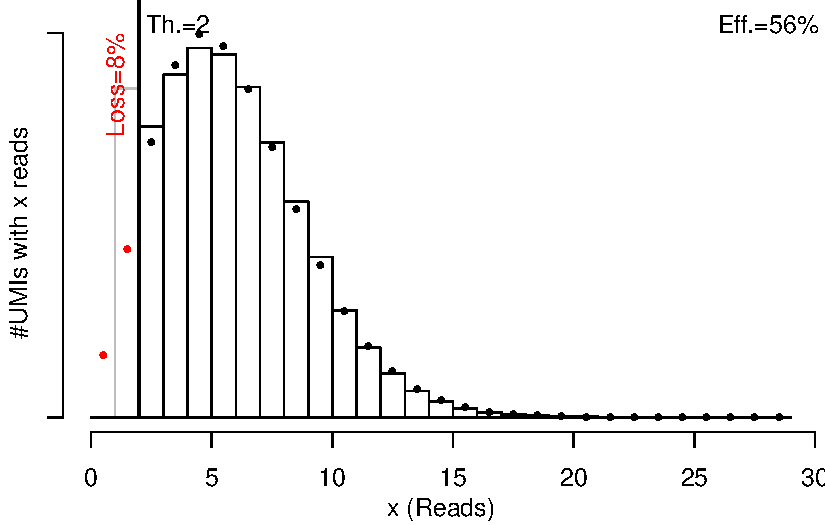
\includegraphics[width=0.45\textwidth,page=1]{../examples/kv_1000g.pdf}\hfill
\includegraphics[width=0.45\textwidth,page=2]{../examples/kv_1000g.pdf}
\\}
\caption*{\textbf{\texttt{kv\_1000g.pdf}}. \texttt{kv\_1000g.bam} processed in single-end mode.}
\end{figure}

\subsection{Paired-End Data with strand UMIs}

The file \texttt{sg\_100g.bam} contains a reduced (restricted to the first 100 genes, and subsamples to 25\%) version of data published by Shiroguchi \textit{et al.}\footnote{Shiroguchi, K., Jia, T. Z., Sims, P. A. \& Xie, X. S. Digital RNA sequencing minimizes sequence-dependent bias and amplification noise with optimized single-molecule barcodes. \textit{Proceedings of the National Academy of Sciences of the United States of America} \textbf{109}, 1347-1352 (2012).} which uses \emph{strand UMIs} (see \nameref{strand-umis} for details).

\subsubsection*{Filtering out incomplete strand UMI pairs}

\shellscript{../examples/sg_100g.cmd}

This command uses UMI-Tools to read (error-corrected) UMIs and their read counts from \texttt{sg\_100g.bam} (\ddarg{input-bam}) containing paired-end reads (\ddarg{paired}), removes UMIs whose partner corresponding to the initial molecule's other strand was not detected (\ddarg{filter-strand-umis}, \ddarg{umipair-sep}) or who have fewer than 24 reads (\ddarg{threshold}), compute gene-specific loss estimates assuming a single initial copy of each UMI (\ddarg{molecules}), writes the bias-corrected counts to \texttt{sg\_100g.tab} (\ddarg{output-counts}), and outputs diagnostic plots to \texttt{sg\_100g.pdf} (\ddarg{output-plots}). For the plots, the bin size for the read-count distribution plot is set to 3 (\ddarg{plot-hist-bin}).

\begin{figure}[H]
{\centering
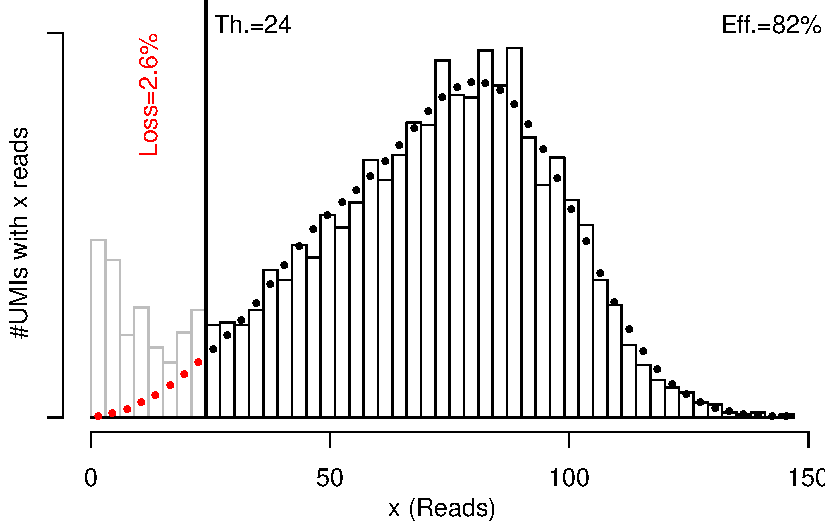
\includegraphics[width=0.45\textwidth,page=1]{../examples/sg_100g.pdf}\hfill
\includegraphics[width=0.45\textwidth,page=2]{../examples/sg_100g.pdf}
\\}
\caption*{\textbf{\texttt{sg\_100g.pdf}}. \texttt{sg\_100g.bam} processed in \emph{filter strand UMIs} mode.}
\end{figure}

\subsubsection*{Combining strand UMIs into pairs}

\shellscript{../examples/sg_100g_comb.cmd}

\enlargethispage{5\baselineskip}
This command uses UMI-Tools to read (error-corrected) UMIs and their read counts from \texttt{sg\_100g.bam} (\ddarg{input-bam}) containing paired-end reads (\ddarg{paired}), combines strand UMIs into UMI pairs (\ddarg{combine-strand-umis}, \ddarg{umipair-sep}), filters UMI pairs with fewer than 24 reads of either strand UMI(\ddarg{threshold}), computes gene-specific loss estimates assuming a single initial copy of each strand UMI (\ddarg{molecules}), writes the bias-corrected counts to \texttt{sg\_100g.tab} (\ddarg{output-counts}), and outputs diagnostic plots to \texttt{sg\_100g.pdf} (\ddarg{output-plots}). For the plots, the bin size for the read-count distribution plot is set to 3 (\ddarg{plot-hist-bin}).

\begin{figure}[H]
{\centering
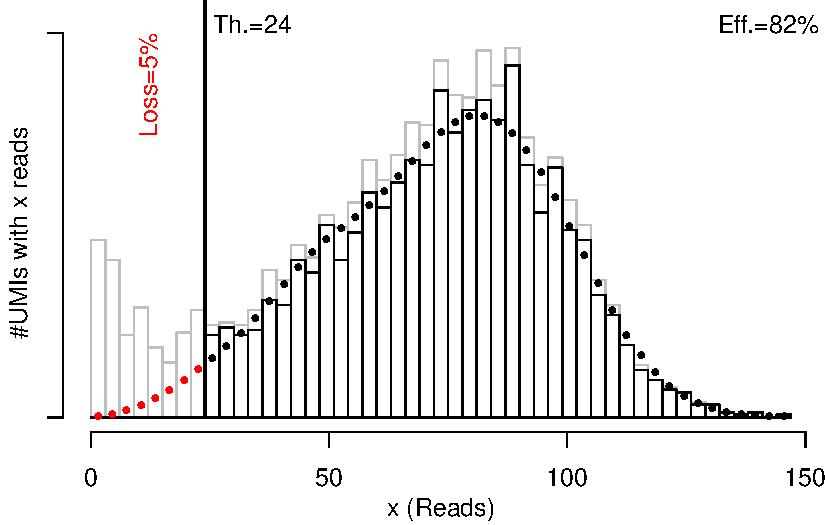
\includegraphics[width=0.45\textwidth,page=1]{../examples/sg_100g_comb.pdf}\hfill
\includegraphics[width=0.45\textwidth,page=2]{../examples/sg_100g_comb.pdf}
\\}
\caption*{\textbf{\texttt{sg\_100g\_comb.pdf}}. \texttt{sg\_100g.bam} processed in \emph{combine strand UMIs} mode. Plots show individual strand UMIs, not UMI pairs. Phantoms now appear even beyond the threshold, because strand UMIs are also considered phantoms if their \emph{partner UMI} has a read count below the threshold.}
\end{figure}

\subsection{Single-cell Data}

The file \texttt{10xn9k\_10c.bam} contains a reduced (restricted to 10 individual cells) version of the \emph{9k Brain Cells from an E18 Mouse}\footnote{\url{https://support.10xgenomics.com/single-cell-gene-expression/datasets/2.1.0/neuron_9k}} public dataset provided by 10x Genomics. 

\shellscript{../examples/10xn9k_10c.cmd}

This command uses UMI-Tools to read (error-corrected) UMIs and their read counts from \texttt{10xn9k\_10c.bam} (\ddarg{input-bam}), removes UMIs with fewer than 2 reads (\ddarg{threshold}), compute gene-specific loss estimates for each combination of gene and cell (\ddarg{group-per}) assuming a single initial copy of each UMI (\ddarg{molecules}), writes the bias-corrected counts to \texttt{10xn9k\_10c.tab} (\ddarg{output-counts}), and outputs diagnostic plots to \texttt{10xn9k\_10c.pdf} (\ddarg{output-plots}). 

UMIs are group disregarding the mapping position, i.e. identical UMI sequences found within the same gene are assumed to belong to the same original molecule (\ddarg{umitools-option} \ddarg{per-gene}). The gene a particular read belongs to is read from the read's XF tag in the BAM file (\ddarg{umitools-option} \ddarg{gene-tag=XF}).

\begin{figure}[H]
{\centering
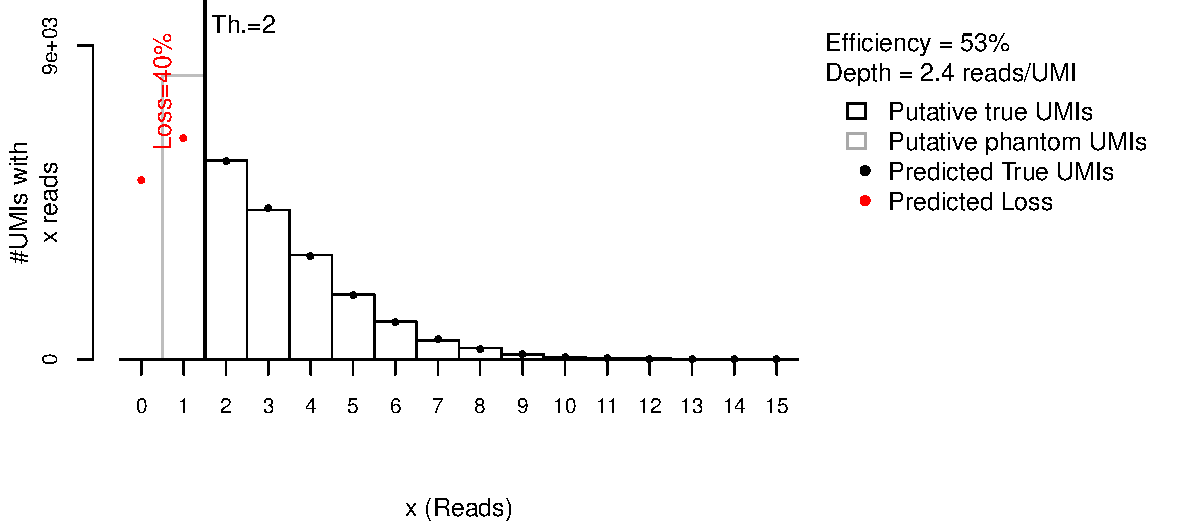
\includegraphics[width=0.45\textwidth,page=1]{../examples/10xn9k_10c.pdf}\hfill
\includegraphics[width=0.45\textwidth,page=2]{../examples/10xn9k_10c.pdf}
\\}
\caption*{\textbf{\texttt{10xn9k\_10c.pdf}}. \texttt{10xn9k\_10c.bam} processed with ``\ddarg{group-per cell,gene}''.}
\end{figure}

\section{License}
TRUmiCount is free software: you can redistribute it and/or modify
it under the terms of the GNU Affero General Public License as published by
the Free Software Foundation, either version 3 of the License, or
(at your option) any later version.

TRUmiCount is distributed in the hope that it will be useful,
but WITHOUT ANY WARRANTY; without even the implied warranty of
MERCHANTABILITY or FITNESS FOR A PARTICULAR PURPOSE.  See the
GNU Affero General Public License for more details.

You should have received a copy of the GNU Affero General Public License
along with TRUmiCount.  If not, see \url{http://www.gnu.org/licenses/}.

\end{document}
